
\begin{figure*}
	\center
	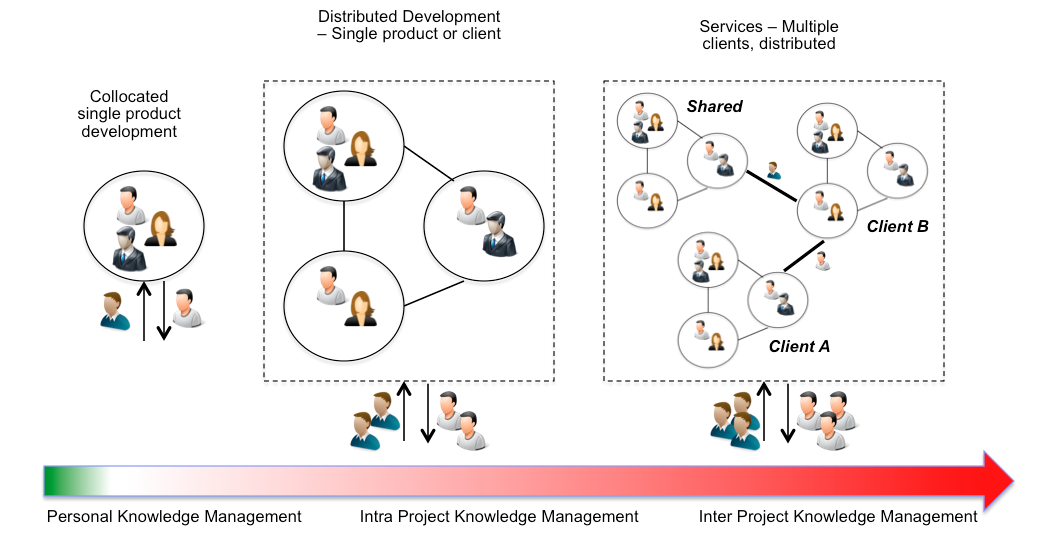
\includegraphics[scale=0.7]{figs/km-types.png}
	\caption{Team structures and knowledge management needs}
	\label{fig-km}
\end{figure*}

\section{Knowledge Management}
\label{sec:km}

Software development is inherently a knowledge intensive activity. Software designers and developers leverage their software development skills along with knowledge about the domain, past experiences and knowledge of team members, to solve the current problem at hand, be it implementing a new feature/application or solving a bug. 
In small, colocated teams too, knowledge management is not a big challenge. Who is an expert on what part of the system is typically known. New team members coming in would use informal channels of communication to figure out who are the experts on the system. If need be, individuals can tap into the knowledge of these experts to quickly address task at hand. 

Knowledge management starts to become a challenge when team size increases and/or teams start getting distributed geographically. In large teams or distributed environments, the requisite knowledge of the system---expertise, dependencies, best practices and so on---is spread across multiple people, locations and even organizations (in cases such as outsourcing) \cite{Desouza:2006}. In such projects, a knowledge management system is needed to create so called project memories that primarily help with following needs. Firstly, they enable new joinees to understand the project with little face to face guidance. Help them identify experts in the project who they can reach out to in case they have queries. Secondly, they enable existing team members to identify artifacts relevant for their current task and people they might need to coordinate with. 

Now consider the case for services organizations such as IBM that are in the business of developing and managing software systems for multiple clients. Day in and day out different employees are churning out new features, resolving issues, implementing new applications for different clients. While each client is different, there is ample scope of reusing best practices and even solutions from past engagements to achieve greater efficiency and efficacy in present and future projects. Consider the following example, for client A there is a need to implement a payroll system. Before starting the project, it would be beneficial to know if a similar system was implemented for some other client, what were the design considerations and challenges faced and if the complete solution could be reused in whole or parts. As another example consider the following scenario, developer Foo has been asked to fix an issue related to leave planning on an application implemented using SAP's Human Capital Management (HCM) module. It so happens that HCM implementation has been done for multiple clients by the organization. It could potentially help Foo if he were to know if similar issue was reported in any other implementations and how it was resolved. At an organization level there is again a need for a knowledge management solution to can act as organization memory \cite{Stein:1995} that helps quickly identify if a similar task (where a task could be a bug to be resolved, an application to be developed or a project risk that needs to be addressed) has been done for another client and if yes, what parts of solution could be reused.

As illustrated in figure~\ref{fig-km}, services organizations need to manage knowledge at all three levels: personal, project and organization. It is believed that individuals are adept at managing their own knowledge and drawing upon it when a new situation comes in \cite{Bruce:2005}. For example, a developer who has been assigned a bug on a system (s)he has implemented would typically know where to start investigation from because of prior knowledge about the system. A project manager working long enough in the product would know the primary risks associated with the project, fault prone areas and so on. However, system support is needed (in form of tools and processes) to effectively manage knowledge at project and organization level primarily because of number of people involved, diversity in their experience and skill levels, geographical distribution and large amount of resource churn.  

In the section we first highlight a couple of existing knowledge management systems. We then discuss then discuss some future research directions in this area.  

\subsection{Examples}
\begin{itemize}
\item Codebook/Hipikat - example of project memory
\item Consultant's Assistant - KM at solution level (example of project memory)
\item Wisdom - KM for troubleshooting
\end{itemize}

\subsection{Research Directions}
\begin{itemize}
\item Auto-codification and personalization
\item Contextual Search
\item Incentives for reuse
\end{itemize}
